\documentclass[a4paper,12pt]{report}

\usepackage[french]{babel}
\usepackage[T1]{fontenc}
\usepackage[utf8]{inputenc}
\usepackage{lmodern}
\usepackage{microtype}

\usepackage{graphicx}
\graphicspath{ {figures/} }
\usepackage{array}

\usepackage{hyperref}

%%%%%%%%%%%%%%%%%%%%%%%%%%%%%%%%%%%%%%%%%%%%%%%%%%%%%%%%
\begin{document}
    %%%%%%%%%%%%%%%%%%%%%%%%%%%%%%%%%%%%%
    %%
    %% Page de Garde
    %%
    %%%%%%%%%%%%%%%%%%%%%%%%%%%%%%%%%%%%%

    \begin{titlepage}
        % En tete 
        \begin{center}
            {\Large ÉCOLE SUPÉRIEURE D’INFORMATIQUE SALAMA}\\
            {\large République Démocratique Du Congo}
            
            {\large Province de Haut-Katanga}
            
            {\large Lubumbashi}
            
            {\large www.esisalama.org}
            \vspace{10pt}
            
            \rule[30pt]{300pt}{1pt}
        \end{center}
        % Logo
        \begin{center}
            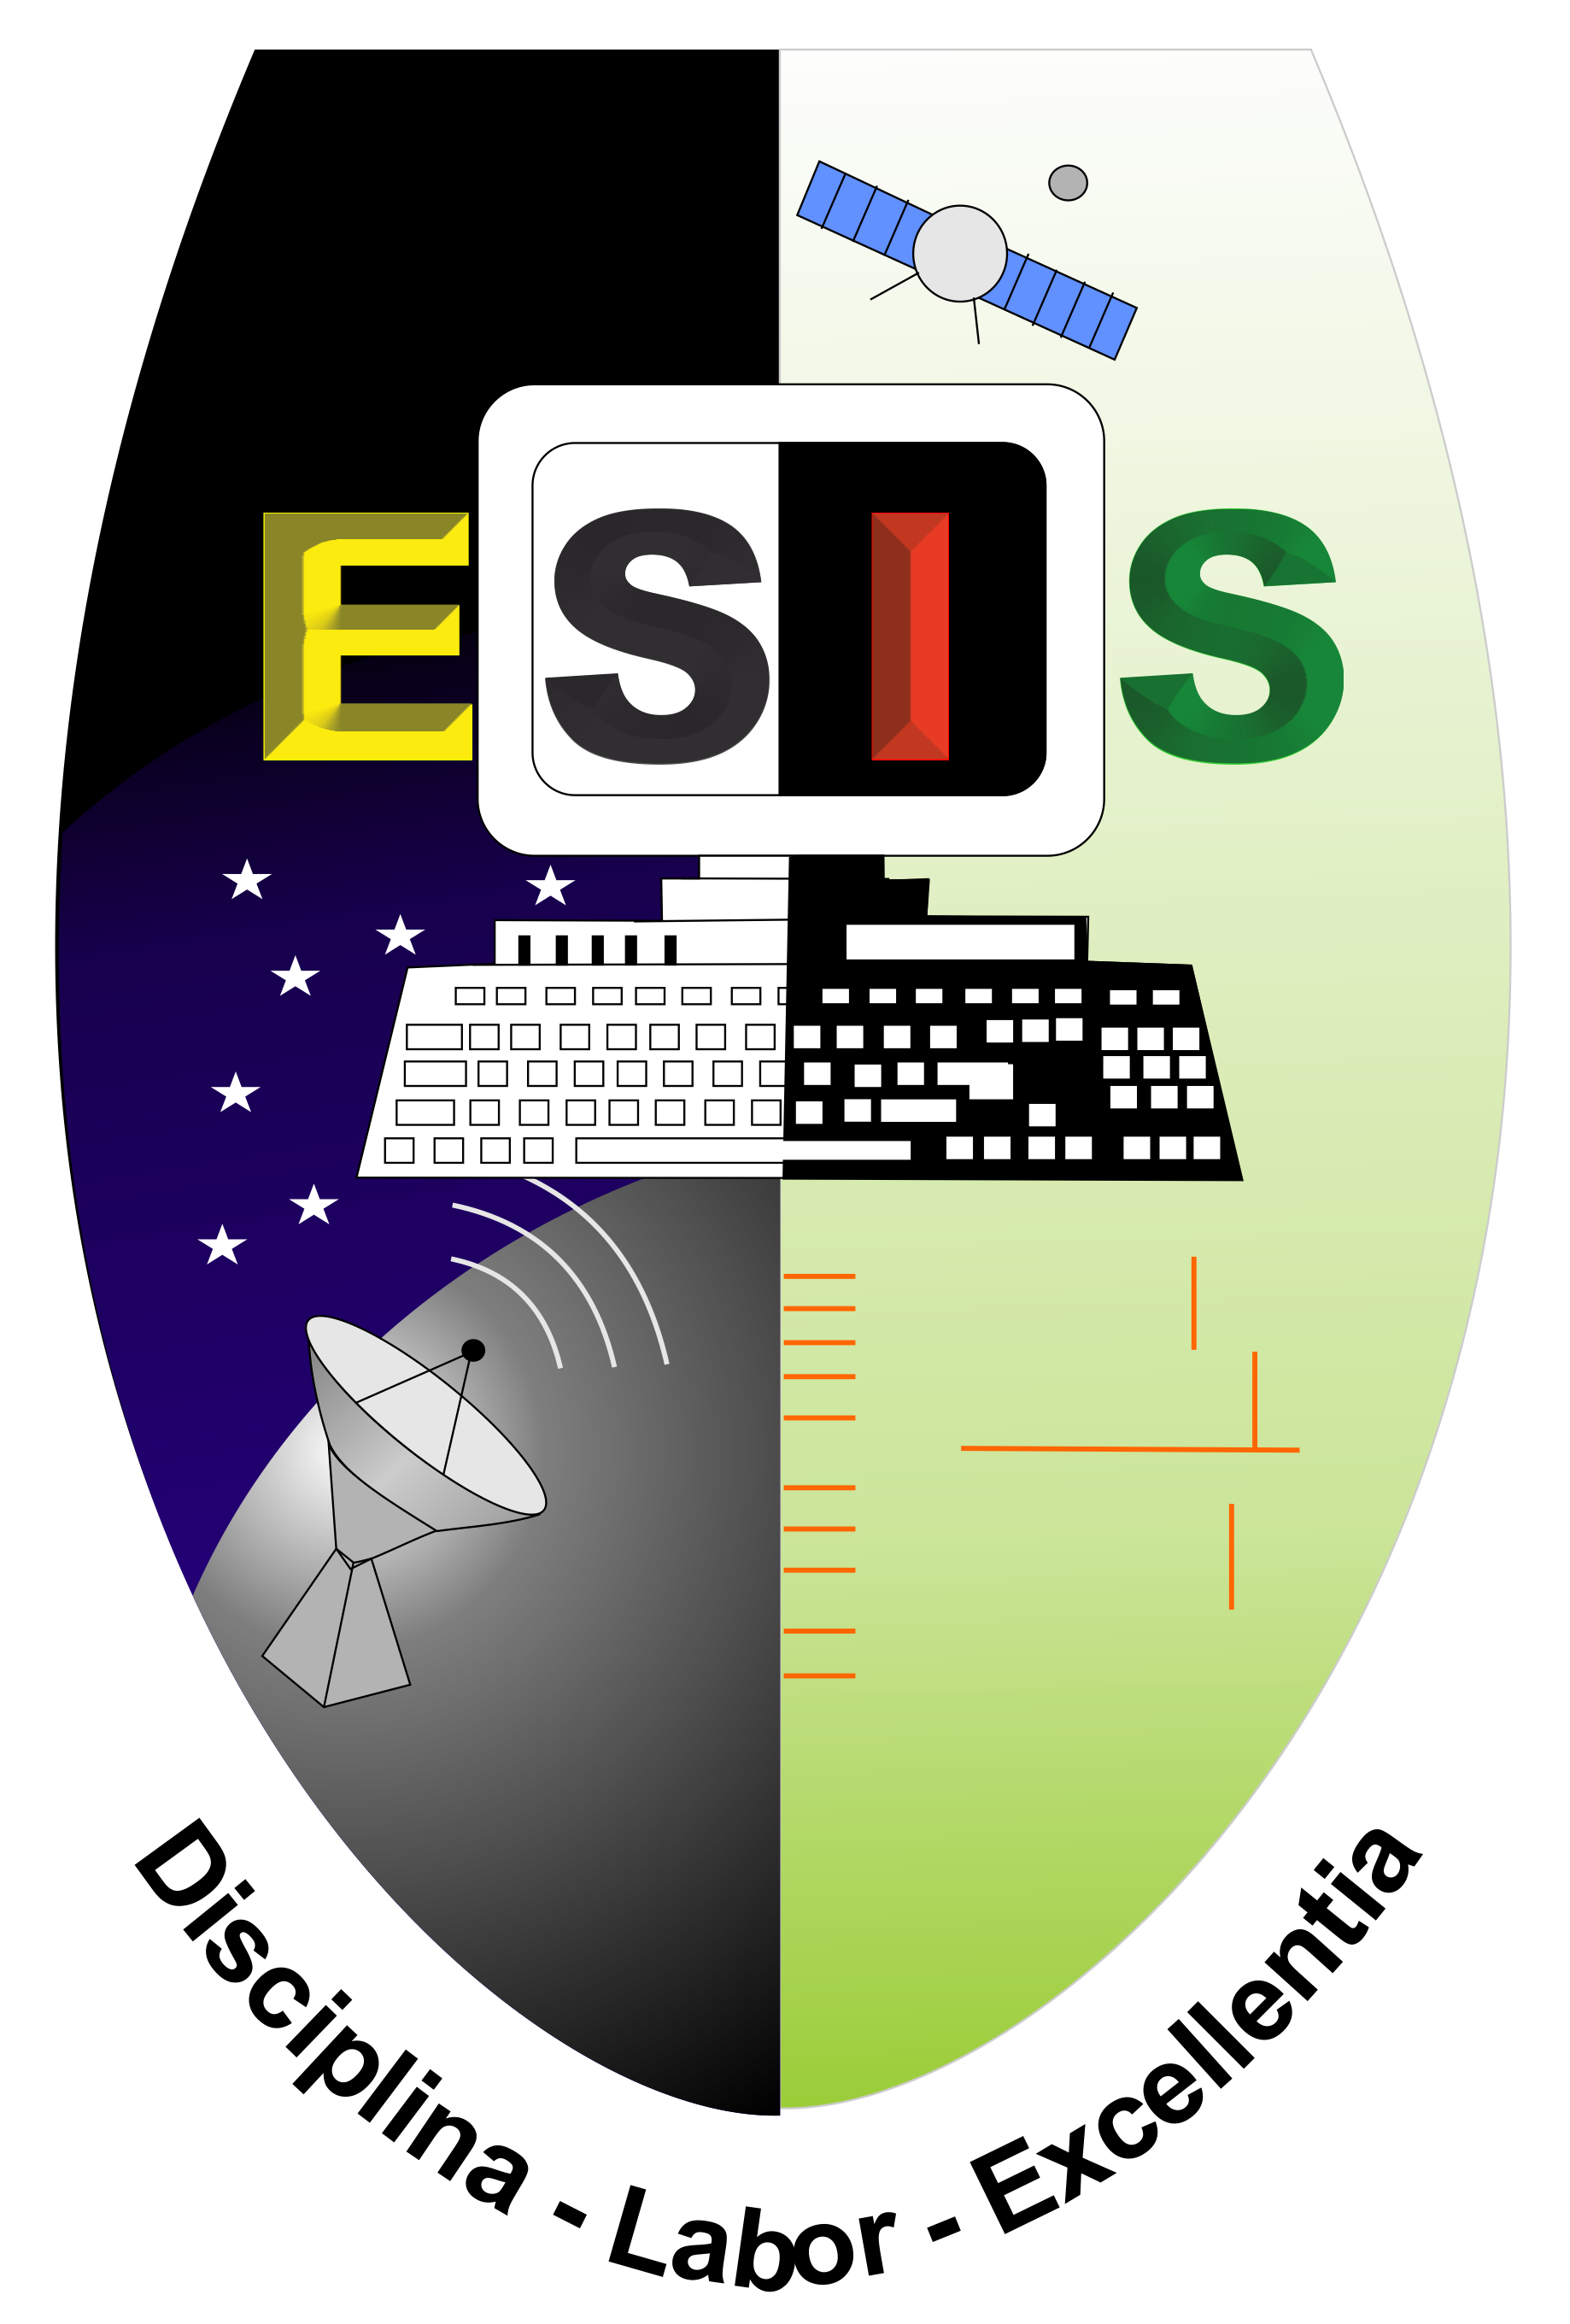
\includegraphics[width=100]{images/logo.png}
        \end{center}
        
        \vspace{15px}

        \begin{center}
            
            \rule[10pt]{\textwidth}{1pt}
            {\LARGE IMPLÉMENTATION DU FLUENT DESIGN AVEC FLUTTER }
            \bigskip
            % \hspace{10pt}
            \rule[10pt]{\textwidth}{1pt}
        \end{center}

        \begin{flushright}
            \small{
                Travail présenté et défendu en vue de l’obtention\\ du grade
            d’ingénieur technicien en Génie Logiciel .  
            }
            
        \end{flushright}

        \hspace{10pt}

        \begin{flushright}
            \textbf{\em{ {\small Par : KABULU MBOLELA Jean Luc}}}
            \\
            \textbf{\em{ \small{Option : Génie Logiciel }}}
        \end{flushright}
        \hspace{5pt}
        \begin{flushright}
            \textbf{\em{ {\small Directeur : Père KAMIBA Isaac }}}
            \\
            \textbf{\em{ \small{Co-directeur : MUKANDA KENGWE Henrique}}}
        \end{flushright}

        \vspace{30pt}
        \begin{center}
           {\large Mars 2020}
        \end{center}

    \end{titlepage}

    \newpage
    
    \begin{center}
        \Huge{IMPLÉMENTATION DU FLUENT DESIGN AVEC FLUTTER}
        \\
        \vspace{15pt}
        \large{KABULU MBOLELA Jean Luc}
        \\
        \vspace{10pt}
        \large{Génie Logiciel}
        \\
        \large{ESIS 2019-2020}
    \end{center}

    \newpage

    %%%% Épigraphe
    

    \begin{center}
        % {\huge \textbf{Épigraphe}}
        \chapter*{Épigraphe}
        \addcontentsline{toc}{chapter}{Épigraphe}
        \vspace{50pt}
         "Celui qui agit d'une main lâche devient pauvre, mais la main des diligents enrichit."
        \begin{flushright}
            Proverbes 10:4, Bible Darby .
        \end{flushright}
    \end{center}

    
    %%%%% Dédicace

    \chapter*{Dédicace}
    \addcontentsline{toc}{chapter}{Dédicace}
    
    \begin{em}
        À mes très chers parents MBOLELA WA KANYANA Patrick \-et CIBOLA Agnes.
        \\
        À mes frères MUKADI MBOLELA Serges, NSONA MBOLELA Cedrick, MUKENGESHAYI MBOLELA Idriss,
        NGOY MBOLELA Daniel et mes sœurs BILONDA MBOLELA Irene, NGALULA MBOLELA Rachel.
        \\
        À ma dulcinée FATIMA FURAHA Espérance.    
    \end{em}
        
    

    %%%%%% Remerciements
    
    \chapter*{Remerciements}
    \addcontentsline{toc}{chapter}{Remerciements}
    

    Arrivé au terme de notre cycle de formation d’Ingénieur Technicien à l’Ecole Supérieure d’Informatique Salama, 
    E.S.I.S en sigle, il est de notre devoir d’exprimer notre gratitude aux personnes qui nous ont aidé à 
    arriver là où nous en sommes aujourd’hui et à réaliser ce travail.
    \\
    C’est ainsi qu’en premier lieu, nous remercions le seigneur Dieu.
    \\
    
    Nos remerciements s’adressent à tout le corps administratif et professoral de l’Ecole
    Supérieure d’Informatique Salama pour avoir concouru à notre formation.
    \\

    De manière particulière au Père KAMIBA Isaac et à Monsieur MUKANDA KENGWE Henrique,
    en leurs qualités respectives de Directeur et Co\-directeur de notre travail.
    \\

    À mes très chers parents MBOLELA Patrick et CIBOLA Agnes.
    \\

    À mon mentor le pasteur Roland DALO.
    

    À mes frères MUKADI MBOLELA Serges, NSONA MBOLELA Cedrick, MUKENGESHAYI MBOLELA Idriss,
    NGOY MBOLELA Daniel et mes sœurs BILONDA MBOLELA Irene, NGALULA MBOLELA Rachel.
    \\

    À tous nos compagnons de lutte avec qui nous avons passé notre parcours
    académique. Allusion faite à : BILEU KAPEPULA Shekina, KYUNGU LUPUNDU Dan, ILUNGA LUBABA Nathan, MANANG KAFUTSHI Elsa, KASY NDIJI Laura, 
    AMPIRE BIGOMOKERO Eric et à toute la promotion 2019-2020 de G3 Génie Logiciel.
    \\

    À mes amis : NGALULA KALENDA Jenny, NGOIE MULOLO Carel et BILEU KAPEPULA Shekina.
    \\

    À tous mes frères et sœurs, neveux et nièces, amis et connaissances dont les noms
    ne sont pas cités, mais que nous portons chaleureusement dans notre cœur.
    Trouvez ici, l’expression de ma profonde gratitude.

    \newpage

    %%%%%% Liste des figures
    \listoffigures
    \newpage

    %%%%%% Liste des tableaux
    \listoftables
    \newpage

    %%%%% Table des matières
    \tableofcontents
    \newpage

    %%%%% Avant-Propos
    \chapter*{Avant-Propos}
    \addcontentsline{toc}{chapter}{Avant-propos}
    Ce travail rentre dans le cadre de l’obtention du diplôme d'ingénieur en Génie Logiciel. 
    Il montrera comment nous sommes parvenus aa trouver une solution à l'utilisation du Fluent Design lors du développement des applications mobiles. L’idée de ce travail de fin de cycle est venue du constat que les développeurs passent beaucoup à concevoir des interfaces graphiques des applications, mais qui, souvent ne respectant les principes d'ergonomie.
    
    
    En Effet, depuis 2018, l'utilisation de Flutter semble augmenter d'une façon étonnante, les développeurs migre de plus en plus vers l'utilisation de Flutter à cause de sa facilite en conception mobile moderne. 
    Flutter est devenu la nouvelle solution de developpement des applications mobiles soit Android ou encore iOS. Entre Temps Flutter, apporte une expérience mobile plus simples et plus moderne dans l'utilisation des applications mobiles.
    Ce travail se veut être une contribution devant permettre de mettre en relief les différents obstacles, mais aussi les avantages d'utilisation de Fluent Design avec Flutter. Ainsi, une bibliothèque est proposée pour lever ces obstacles, en particulier sur Android et sur iOS.
    
    
    Des difficultés n’ont pas manqué. Elles concernent particulièrement la disponibilité de données fiables et actuelles. Elles concernent également la disponibilité des designers qui prennent les décisions dans la conception des applications mobiles pour la réalisation d’interview. Cette dernière situation nous a obligé à nous contenter des entretiens informels que nous avons pu avoir avec quelques spécialistes.

    \vspace{20px}
    \begin{flushright}
        Ce document a été traité avec \LaTeX
    \end{flushright}
    
    %%%%%% Introductio
    \chapter*{Introduction}
    \addcontentsline{toc}{chapter}{Introduction}

        \section*{Problématique}
        \addcontentsline{toc}{section}{Problématique}

            \subsection*{Situation de la problématique}
            \addcontentsline{toc}{subsection}{Situation de la problématique}

                De nos jours, les utilisateurs de téléphones portables attendent de leurs applications un beau design, 
                des animations fluides et de grandes performances. 
                De plus en plus avec le développement en intégration continue qui oblige aux entreprises ou des 
                startups des développement des applications de publier d’une manière constante les mises a jours .

                
                Entre temps pour permettre aux utilisateurs des applications mobiles d’avoir plus des facilité et plus 
                d'intuition, de grandes Firmes telle que Microsoft, Google ou Samsung font des études approfondies sur 
                le comportement humains pour savoir comment ils réagissent face une applications mobiles, 
                Comment ils comprennent différentes icônes, comment ils déplacent leurs doigts sur l'écran , 
                comment ils réagissent devant certaines couleurs.
        
                Depuis Décembre 2019, Microsoft a lancé "Fluent Design System" \footnote{https://www.microsoft.com/design/fluent/} ,un ensemble des principes fondamentaux 
                de Design pour aider les concepteurs et développeurs à construire et concevoir des produits 
                pour leur clients  visant à créer de la simplicité et de la cohérence grâce à un système de conception 
                partagé et ouvert sur toutes les plateformes.
        
                Fluent Design est un système de design collective et ouverte qui garantit que les personnes, 
                les équipes et leurs produits disposent des composants et des processus fondamentaux pour créer 
                des expériences utilisateurs cohérentes sur toutes les plateformes.
        
            \subsection*{Problème de la recherche}
            \addcontentsline{toc}{subsection}{Problème de la recherche}
                Les problèmes que nous avons rencontré est que les développeurs manque du code qui contient l’ensemble des
                 principes et des outils ( tels que la typographie, les couleurs, Les contrôles, Les animations )  
                 qui permet d'implémenter le Fluent Design dans leur applications mobiles.

            \subsection*{Question de la recherche}
            \addcontentsline{toc}{subsection}{Question de la recherche}
                En lisant les lignes qui précèdent, la question suivante peut être soulevée :
                
                \begin{itemize}
                    \item comment concevoir une applications avec moins de code pour avoir une application 
                    qui respecte l'aspect visuel de Fluent Design ?
                \end{itemize}
        
        \section*{Hypothèses}
        \addcontentsline{toc}{section}{Hypothèses}

            Face à ce problème auquel se confronte les développeurs, principalement les développeurs des applications mobiles 
            qui aimerait utiliser le fluent Design, nous avons  mis au point une bibliothèque native qui fournit 
            l'expérience de l'interface utilisateur de Microsoft pour la plate-forme Android.
            pour y parvenir notre bibliothèque apporte du style pour les boutons, les formulaires, 
            la navigation… Il permet ainsi de concevoir une application mobiles rapidement et avec peu de 
            lignes de code ajoutées.
        
        \section*{Choix et Intérêt du sujet}
        \addcontentsline{toc}{section}{Choix et Intérêt du sujet}
            
            \subsection*{Choix du sujet}
            \addcontentsline{toc}{subsection}{Choix du sujet}
                Comme le stipule le vad mecum de notre institut , 
                a la fin  du premier cycle à l'ecole supérieure d'informatique Salama, 
                il est demander de resoudre un probleme autour comme travail de fin de cycle.
                Notre choix a porté sur « L'implémentation du Fluent Design avec Flutter » 
                dans le but de faciliter le développement des applications mobiles.
            
            \subsection*{Intérêt du sujet}
            \addcontentsline{toc}{subsection}{Intérêt du sujet}

                \subsubsection*{Intérêt Personnel}
                \addcontentsline{toc}{subsubsection}{Intérêt Personnel}
                    Étant Largement passionné par le développement mobile et très émerveillé par la technologie Flutter \footnote{Flutter est le framework d'interface utilisateur de Google qui permet de créer de belles applications nativement compilées pour le mobile, le web et le pc à partir d'une seule base de code.} \footnote{http://flutter.dev/}, 
                    qui est devenu est une technologie phare et populaire, 
                    nous avons décidé de contribuer avec une bibliothèque qui aidera la communauté des développeurs mais aussi 
                    dans le but d'approfondir ma connaissance sur Flutter.
                
                \subsubsection*{Intérêt scientifique}
                \addcontentsline{toc}{subsubsection}{Intérêt scientifique}
                    Nous avons opté pour ce sujet afin de répondre aux exigences académiques fixées à tout étudiant finaliste, 
                    celui de réaliser un travail de fin de cycle. Mais l’obtention d’un diplôme n’est pas le seul l'intérêt de ce travail, 
                    car nous le voulons aussi pour contribuer aux développement et l'évolution du Framework Flutter.  
                    Nous voudrions que ce travail 
                    soit un ajout nécessaire qui permettra de développer plus rapidement les applications mobiles avec Flutter.
            
            \section*{Méthode}
            \addcontentsline{toc}{section}{Méthode}
                Une bonne méthodologie permet de structurer les démarches à suivre de façon à ce que l’etudiant puisse évoluer 
                dans le temps, en suivant les jalons importants aussi bien pour les travaux de recherches que pour la 
                rédaction du travail.

                Pour notre travail, nous avons opté pour la méthode nommée UP \footnote{UP : Unified Process},
                Le processus unifié est un processus de développement logiciel itératif, centré sur l'architecture, 
                piloté par des cas d'utilisation et orienté vers la diminution des risques.
            
            \section*{Techniques}
            \addcontentsline{toc}{section}{Techniques}
                Pour notre notre travail nous avons utilisé les techniques suivantes :
                \begin{itemize}
                    \item Documentaire qui consiste essentiellement à consulter des livres, 
                          des notes de cours, des documentations sur internet, des travaux de fin de cycle, 
                          des thèses soutenues et des articles voir des vidéos disponibles sur les différentes plateformes 
                          d’enseignements en ligne
                \end{itemize}

            

\end{document}